\chapter*{Marco teórico}\label{ch:marcoteorico}
\addcontentsline{toc}{chapter}{Capitulo 3. Marco teórico}
\section{Marco teórico}
En este capítulo, se explicarán los conceptos utilizados en el método propuesto que se desarrollará en el presente trabajo de tesis, estructurados en cinco grandes aristas: sitios de CQA, Sistemas de Recomendación, Big Data y medidas de similaridad y clustering. Todos estos conceptos se combinarán para luego, en el siguiente capítulo, desarrollar un método que satisfaga los objetivos del trabajo de tesis, de una manera superadora.

\subsection{Sitios de CQA}
Los servicios de Community Question Answering CQA, son un tipo especial de servicios de \textit{Question Answering} (QA), los cuales permiten a los usuarios registrados responder a preguntas formuladas por otras personas. Los mismos atrajeron a un número creciente de usuarios en los últimos años \citep{li2010routing}. Una pregunta formulada en Quora, y respondida por su fundador y CEO, Adam D'Angelo, revela que el sitio recibe más de 200 millones de visitantes únicos mensualmente (información actualizada a Junio de 2017), lo que denota la popularidad de este tipo de portales\footnote{Pregunta formulada en el sitio Quora “How many people use Quora?”: \url{https://www.quora.com/How-many-people-use-Quora-3}. Último acceso: Febrero 2021.}. Desde la creación de este tipo de servicios, se han aplicado diferentes técnicas de software para que los usuarios encuentren respuestas a sus preguntas en el menor tiempo posible y aprovechar al máximo el valor de las bases de conocimiento, por ejemplo, un framework para predecir la calidad de las respuestas con características no textuales \citep{jeon2006framework}, incorporar información de legibilidad en el proceso de recomendación \citep{anuyah2017can}, encontrar a los expertos apropiados \citep{li2010routing}, o recomendar la mejor respuesta a una pregunta dada, entre otros. Sin embargo, el mecanismo existente en el cual se responden las preguntas en los sitios de CQA todavía no alcanza a satisfacer las expectativas de los usuarios por varias razones: \begin{enumerate*} [label=(\roman*)] \item baja probabilidad de encontrar al experto: una nueva pregunta, en muchos casos, puede no encontrar a la persona con la habilidad de responder de manera correcta, resultando en respuestas tardías y que distan de ser óptimas; \item respuestas de baja calidad: los sitios de CQA suelen contener respuestas de baja calidad, maliciosas y spam. Estas suelen recibir baja calificación de los miembros de la comunidad; \item preguntas archivadas y poco consultadas: muchas preguntas de los usuarios son similares.\end{enumerate*} Antes de formular una pregunta, un usuario podría beneficiarse de buscar ya formuladas, y por consiguiente, sus respuestas \citep{yang2013cqarank}.

\subsection{Sistemas de recomendación}
\subsubsection{Contexto Histórico}
Es muy frecuente tener que tomar decisiones sin la suficiente experiencia personal sobre las alternativas disponibles. En la vida cotidiana, confiamos en recomendaciones de otras personas ya sea de boca en boca o cartas de recomendación, reseñas de libros y películas o encuestas generales. Los sistemas de recomendación asisten este proceso natural en el ámbito de los sistemas de información \citep{resnick1997recommender}. El primer RS, Tapestry \citep{goldberg1992using}, fue un sistema experimental de correo electrónico destinado a resolver el problema de manejar grandes cantidades de emails filtrando según cuán interesantes son los documentos, utilizando un enfoque basado en el contenido de los mismos y también filtros colaborativos, lo que después se denominaría RS no personalizados y personalizados por Ricci, Rokach y Shapira en el año 2011. Se ha trabajado mucho en mejorar y desarrollar nuevos enfoques con respecto a RS en los últimos años, y el interés en esta área sigue vigente debido a la abundancia de aplicaciones prácticas en las cuales es necesario ayudar a los usuarios a lidiar con la sobrecarga de información\footnote{El concepto de sobrecarga de información, del inglés information overload, hace referencia a cuando los usuarios reciben demasiada información, por lo cual, la precisión en sus decisiones empieza a decrecer \citep{eppler2004concept}.} y proveer recomendaciones personalizadas, contenidos y servicios. Sin embargo, a pesar de todos estos avances, la generación actual de RS todavía requiere mejoras para que los métodos de recomendación sean más efectivos y aplicables a una gama más amplia de sistemas y/o sitios. Aunque las raíces de los RS se remontan a trabajos en ciencia cognitiva \citep{rich1979user}, teoría de aproximación \citep{powell1981approximation}, recuperación de información \citep{salton1989automatic}, ciencias de las predicciones \citep{armstrong2001principles}, ciencias de la gestión \citep{murthi2003role} y también al modelado de la elección de consumidor en marketing \citep{lilien1992marketing}, los RS recién surgen como un área de investigación independiente en la década de 1990, cuando los investigadores comenzaron a centrarse en problemas de recomendación que se basan específicamente en \textit{calificaciones} \citep{adomavicius2005toward}. En su formulación más común, el problema de recomendación se reduce a estimar calificaciones para los ítems que no han sido vistos por un usuario.

\subsubsection{Funciones de un Sistema de Recomendación}
Como se mencionó anteriormente, un RS es un conjunto de herramientas de software que sugiere items a un usuario, que posiblemente utilizará. Haciendo énfasis particularmente en RS comercial, probablemente la función más importante es incrementar el número de ítems vendidos, lo cual es posible porque el RS ofrecerá los ítems sobre los cuales el usuario tiene más probabilidades de querer o necesitar. Esto implica, aumentar el ratio de conversión, es decir, la cantidad de ventas que es posible efectuar sobre un ítem sobre del total de oportunidades que un usuario selecciona el mismo. Por ejemplo, en un sitio de delivery de comida online, cuantas veces un usuario realiza un pedido en un restaurante en particular, sobre el total de veces que observó el menú del mismo. Indudablemente, la conversión va a ser mayor si el usuario recibe recomendaciones de restaurantes que están más cercanos a su gusto personal. Otra función de un RS comercial muy relacionada a la anterior es vender productos más diversos, ya que sería muy difícil para un usuario encontrarlos sin una recomendación precisa.

\bigskip Desde el punto de vista del usuario, un conjunto de recomendaciones precisas y relevantes aumentarán su satisfacción y fidelidad. El usuario disfrutará usar un sistema donde cada ítem o característica que utiliza está diseñada teniendo en cuenta sus intereses. Aumentar la fidelidad del usuario con el sitio, significa que habrá mucha más interacción y, por lo tanto, el modelo de recomendación se volverá más refinado; pudiendo utilizar este conocimiento para mejorar otros sistemas relacionados, como control de stock o publicidad \citep{ricci2011introduction}.

\subsubsection{Técnicas de Recomendación}
Para implementar su función principal, un RS debe \textit{predecir} si vale la pena recomendar un ítem en particular. Para esto, este sistema debe ser capaz de predecir la utilidad de algunos de los ítems, o al menos poder comparar la utilizad entre algunos de ellos, y entonces decidir qué ítems recomendar basándose en esta comparación. Para realizar estas comparaciones, los RS basan sus estrategias de recomendaciones en 6 técnicas básicas \citep{ricci2011introduction}:

\paragraph{Basados en contenido}
Los RS basados en contenido intentan recomendar ítems similares a los que el usuario eligió anteriormente. Como su nombre lo indica, el proceso básico llevado a cabo por estos RS consiste en hacer coincidir atributos del perfil de usuario que posean preferencias e intereses en la búsqueda actual, con los atributos del ítem que se va a recomendar \citep{lops2011content}. Este tipo de RSs es especialmente útil cuando se conocen características de los ítems a recomendar pero no se conocen características del usuario, en otras palabras, estos sistemas intentan recomendar ítems similares a los que el usuario ha elegido anteriormente.

\bigskip Uno de los limitantes conocidos de estos RS es que son limitados a recomendar ítems del mismo tipo al que el usuario está solicitando. Por ejemplo, no sería posible recomendar música, utilizando videos ya que el perfil de contenido es distinto. Para solucionar esto, muchos de los RS basados en contenido están utilizando algoritmos híbridos con otro tipo de técnicas de recomendación.

\paragraph{Filtrado Colaborativo}
El \textit{Filtrado Colaborativo} (Collaborative Filtering en inglés o CF) es el proceso de filtrado o evaluación de ítems usando las opiniones de los demás \citep{schafer2007collaborative}. El Filtrado Colaborativo es el enfoque original y el más simple de todas las técnicas de recomendación, y el más utilizado. Se basa en recomendar al usuario activo, los ítems que otros usuarios con gustos similares eligieron en el pasado.

\paragraph{Demográficos}
La mayoría de los RS utilizan enfoques basados en conocimiento o en contenido, esto implica que se necesita la suficiente información o un conocimiento adicional para poder llevar a cabo las recomendaciones. Los RS demográficos hacen recomendaciones basadas en clases demográficas, la ventaja es que la información histórica no es necesaria. Por ejemplo, una aplicación podría ser utilizar información demográfica para predecir el rating de distintos turistas a atracciones, basándose en enfoques predictivos de Machine Learning \citep{wang2012applicability}. Las técnicas demográficas forman correlaciones “personas-a-personas”, como los sistemas colaborativos, pero utilizando distinta naturaleza de los datos, en este caso, el perfil demográfico del usuario.

\paragraph{Basados en conocimiento}
Los RS \textit{basados en conocimiento} (Knowledge-based en inglés), usan el conocimiento acerca de los usuarios e ítems a recomendar para generar la recomendación, razonando acerca de que items satisfacen los requerimientos del usuario \citep{burke2000knowledge}.

\bigskip Los RS de filtrado colaborativo, al utilizar datos de otros usuarios, deben ser inicializados con un conjunto de datos considerablemente grande, ya que un sistema con una base de datos pequeña es improbable que sea útil. Además, la precisión del sistema es muy sensible al número de ítems asociados con un usuario dado \citep{shardanand1995social}. Esto conlleva a un problema de inicialización: hasta que no exista un número considerable de usuarios cuyas elecciones y hábitos sean conocidos, el sistema no será útil para un nuevo usuario.  Lo mismo sucede para los RS que toman enfoques de Machine Learning. Típicamente, este tipo de sistemas se convierten en buenos clasificadores una vez que han aprendido desde una gran base de datos. Los RSs basados en conocimientos evitan estas desventajas. No existe un problema de inicialización, ya que las recomendaciones no dependen de un conjunto de datos grande. Para estos RSs no es necesario recolectar información acerca de un usuario en particular porque las recomendaciones que realizan son exclusivamente basadas en las elecciones de un usuario en particular. Estas características no solo hacen a este tipo de RS muy valioso en sí mismo, sino también como complemento de otros RS que utilicen distintas técnicas.

\paragraph{Basados en comunidades}
Un \textit{RS basado en comunidades} (community-based en inglés) hace uso del método “boca a boca” digital para construir una comunidad de individuos que comparten opiniones personales y experiencias relacionadas con sus recomendaciones de ítems. Estos sistemas, presentan y agregan opiniones generadas por los usuarios en un formato organizado, las cuales son consultadas a la hora de tomar decisiones (por ejemplo, comprar un producto) \citep{chen2009community}. La evidencia sugiere que las personas están más inclinadas para seguir una sugerencia de sus amigos que una sugerencia similar que viene desde una persona anónima \citep{sinha2001comparing}. Este tipo de RS toma importancia cuando se tiene en cuenta la creciente popularidad de las redes sociales abiertas, tal que estos sistemas también son conocidos como \textit{Sistemas de Recomendación Sociales}.

\paragraph{Sistemas Híbridos}
Una variedad de técnicas fueron propuestas como base de los sistemas de recomendaciones. Cada una de ellas, tienen desventajas conocidas, como el ya mencionado problema de inicialización de los sistemas colaborativos y basados en contenido. Un \textit{RS Híbrido} combina múltiples técnicas de recomendación para encontrar sinergia entre las mismas. Por ejemplo, un sistema basado en conocimiento puede compensar el problema de inicialización de los sistemas colaborativos, para nuevos perfiles de usuario; así como también, el componente colaborativo puede utilizar sus habilidades estadísticas para encontrar pares de usuarios que compartan preferencias no esperadas, las cuales no podrían haber sido predichas por habilidades basadas en conocimiento \citep{burke2007hybrid}.
\subsection{Big Data}
\subsubsection{Contexto Histórico}
Al igual que todos los términos que surgen a partir de avances tecnológicos, no existe un consenso claro de cómo definir \textit{Big Data}. \cite{manyika2011big} definen este concepto como los conjuntos de datos cuyo tamaño está más allá de la habilidad de las herramientas software de base de datos para capturar, almacenar, gestionar y analizar. Nótese que esta definición no define un tamaño mínimo del conjunto de datos, sino que asume que la tecnología avanza constantemente como así también las herramientas, por lo cual, la definición se "mueve" con el tiempo. Por otro lado, también es interesante tomar otra arista en la definición de este concepto: la consultora Gartner en su sitio web\footnote{Concepto de Big Data en el glosario de Gartner: \url{https://www.gartner.com/en/information-technology/glossary/big-data}. Último acceso: Febrero 2021.} lo define como "Big Data son activos de información caracterizados por su alto volumen, velocidad y variedad que demandan formas innovadoras y rentables de procesamiento de información para mejorar la compresión y la toma de decisiones", haciendo énfasis en la multiplicidad de características del concepto de Big Data.

\bigskip El comienzo de sobrecarga de información, recientemente mencionado, data del año 1880, cuando el censo de los Estados Unidos tarda 8 años en tabularse. Ante esta situación Herman Hollerith inventó la máquina tabuladora eléctrica basada en tarjetas perforadas\footnote{Herman Hollerith, US Census Boureau: \url{https://www.census.gov/history/www/census_then_now/notable_alumni/herman_hollerith.html}. Último acceso: Febrero 2021.}. El censo en 1890 fue un éxito rotundo e, incluso, la máquina diseñada fue utilizada para los censos de Canadá, Noruega y Austria al año siguiente. En el año 1941, los científicos empiezan a utilizar el término “explosión de la información”, que fuera citado en el periódico The Lawton Constitution\footnote{The Lawton Constitution: \url{http://www.swoknews.com/}.  Último acceso: Febrero 2021.}, haciendo alusión a la dificultad de administrar toda la información disponible. Gradualmente, se identificaron avances concretos en materia de procesamiento de datos y criptografía, motivados particularmente por los sucesos bélicos de la época. Un ejemplo es el dispositivo llamado Colossus \citep{copeland2004colossus} que buscaba e interceptaba mensajes a una tasa de miles de caracteres por segundo. Unos años más tarde, en 1951, el concepto de \textit{memoria virtual} es introducido por el físico alemán Fritz-Rudolf Güntsch, como una idea que trataba el almacenamiento finito como infinito.

\bigskip A partir de la década del 80’, los avances tecnológicos, especialmente en sistemas MRP (planificación de recursos de fabricación), permitieron nuevas formas de organizar, almacenar y generar datos. En este sentido, IBM se destaca y define una arquitectura para los informes y análisis de negocio (EBIS)\footnote{Acrónimo para EMEA (Europe, Middle East and Africa) Business Information System.}, que se convierte en la base del almacenamiento de datos en forma centralizada para usuarios finales \citep{devlin1988architecture}; es decir, el \textit{data warehousing}. Hacia finales de los 80’, Tim Berners-Lee, inventa la \textit{World Wide Web} \citep{berners1992world}, invento que implicaría el impacto más grande hasta la actualidad con respecto a la generación, identificación, almacenamiento y análisis de grandes volúmenes de datos de diversa naturaleza.

\bigskip El inicio de los años 90’ marcan un antes y un después en lo relativo al tratamiento y almacenamiento de datos. El crecimiento tecnológico fue explosivo, tal es así que el almacenamiento digital empieza a ser más conveniente y rentable que el papel para almacenar datos \citep{morris2003evolution}. Es en 1990 cuando surgen las plataformas de \textit{Business Intelligence} (BI) y los rediseños de software al estilo \textit{Enterprise Resource Planning} (ERP). En este contexto, \cite{cox1997application} afirman que el crecimiento de la cantidad de datos que debe manejar un sistema de información empieza a ser un problema en materia de almacenamiento y visualización de los datos, situación que denominaron como “el problema del Big Data”. Así, 1997 es un año clave, en el que se realizan un gran porcentaje de estudios y publicaciones que se enfocan en averiguar cuánta información hay disponible a nivel mundial y su crecimiento\footnote{Michael Lesk publica \textit{“How much information is there in the world?”} (1997): \url{http://www.lesk.com/mlesk/ksg97/ksg.html}. Último acceso: Febrero 2021.} y, en consecuencia, se estima que el crecimiento de Internet es aproximadamente del 100\% anual y que superaría el tráfico de voz para el año 2002 \citep{coffman1998size}.

\bigskip En el año 2001, se introduce el concepto de \textit{Las 3 V’s: Volumen, Velocidad y Variabilidad de los datos} \citep{laney20013d}, fundantes sobre la temática y que sería mundialmente aceptado una década más tarde. Por otro lado, también en 2001, aparece el concepto de \textit{Software como un Servicio} (SaaS) \citep{hoch2001software}, un modelo disruptivo de servicios centralizados y acceso a los mismos mediante clientes finos (típicamente exploradores web), dando la posibilidad del escalamiento horizontal de sistemas de información y la generación de estándares de comunicación. Esta situación provocó que empresas como Oracle\footnote{Oracle: \url{https://www.oracle.com}. Último acceso: Febrero 2021.}, SAP\footnote{SAP: \url{https://www.sap.com}. Último acceso: Febrero 2021.} y Peoplesoft\footnote{Peoplesoft: adquirida por Oracle en Enero de 2005.} empiecen a centrarse en el uso de servicios web, permitiendo así la generación de datos en forma masiva por usuarios finales. Así, en 2006, nace Apache Hadoop\footnote{Apache Hadoop: http://hadoop.apache.org/. Último acceso: Febrero 2021.}, una solución de código abierto que permite el procesamiento en paralelo y distribuido de enormes cantidades de datos en forma escalable. Posteriormente, en 2008, se empieza a pensar al Big Data como la mayor innovación en informática en la última década, ya que ha transformado la forma en que los motores de búsqueda acceden a la información, las actividades de las compañías, las investigaciones científicas, la medicina, y las operaciones de defensa e inteligencia de los países, entre otras tantas actividades. Más aún, se ha comenzado a ver su potencial para recopilar y organizar datos en todos los ámbitos de la vida cotidiana \citep{bryant2008big}, tales como redes sociales, estadísticas deportivas, o avances médicos y genéticos.

\subsubsection{Map-Reduce}
Map-reduce es un modelo de programación popular para el procesamiento de grandes cantidades de datos mediante computación distribuida \citep{condie2010mapreduce}.  En pocas palabras, se especifica una función map que procesa pares clave-valor para generar un conjunto de pares clave-valor intermedios, y una función reduce que combina todos los valores intermedios asociados con la misma clave \citep{dean2008mapreduce}.
En lenguajes de programación funcionales así como también lenguajes de alto nivel modernos, es posible escribir expresiones de estilo lambda, en las cuales es posible paralelizar y ejecutar programas en clusters distribuidos sin la necesidad de tener en cuenta los detalles de partición de datos y subprocesamiento.
\bigskip En este trabajo se utilizará el framework Apache Spark\footnote{Sitio web oficial de Apache Spark: \url{https://spark.apache.org/}. Último acceso: Febrero 2021.}, debido a su poder de procesamiento distribuido, su arquitectura basada en datos y su compatibilidad con las librerías necesarias en este trabajo.

\paragraph{Arquitectura Hadoop}
La librería de software Apache Hadoop es un framework que posibilita el procesamiento de grandes conjuntos de datos entre clusters de computadoras usando modelos de programación simples. Para posibilitar esto, Hadoop se basa en una arquitectura de archivos propia, llamada HDFS\footnote{Siglas en inglés para Hadoop Distributed File System.} (Sistema de Archivos Distribuido Hadoop). En la mayoría de los procesos basados en Hadoop, HDFS es utilizado para almacenar la entrada del paso \textit{map} y la salida del paso \textit{reduce}, pero no los resultados intermedios, ya que ellos se almacenan en el sistema de archivo de cada uno de los nodos \citep{condie2010mapreduce}. Según el sitio oficial\footnote{Arquitectura HDFS: https://hadoop.apache.org/docs/stable/hadoop-project-dist/hadoop-hdfs/HdfsDesign.html. Último acceso: Febrero 2021.}, HSFS es altamente tolerante a fallos y es diseñado para ser ejecutado en computadoras de bajo costo. Además, HDFS provee gran productividad accediendo a los datos de una aplicación y es posible usarlo en grandes conjuntos de datos.

\bigskip HDFS tiene una arquitectura maestro-nodo\footnote{Del inglés, master-node architecture.}. Un cluster HDFS (conjunto de nodos maestro-nodos) consiste en un \textit{NameNode}, que es un servidor maestro que maneja el espacio de nombres del sistema de archivos y regula el acceso a archivos. Además, hay un número de \textit{DataNodes}, usualmente uno por cada nodo en el cluster, que maneja el almacenamiento de datos en archivos. Internamente, un archivo es dividido en uno o más bloques, y esos bloques son almacenados en DataNodes. Por otro lado, el NameNode ejecuta operaciones tales como abrir, cerrar, y renombrar archivos y directorios.
\bigskip
\begin{figure}[h!]
	\centering
	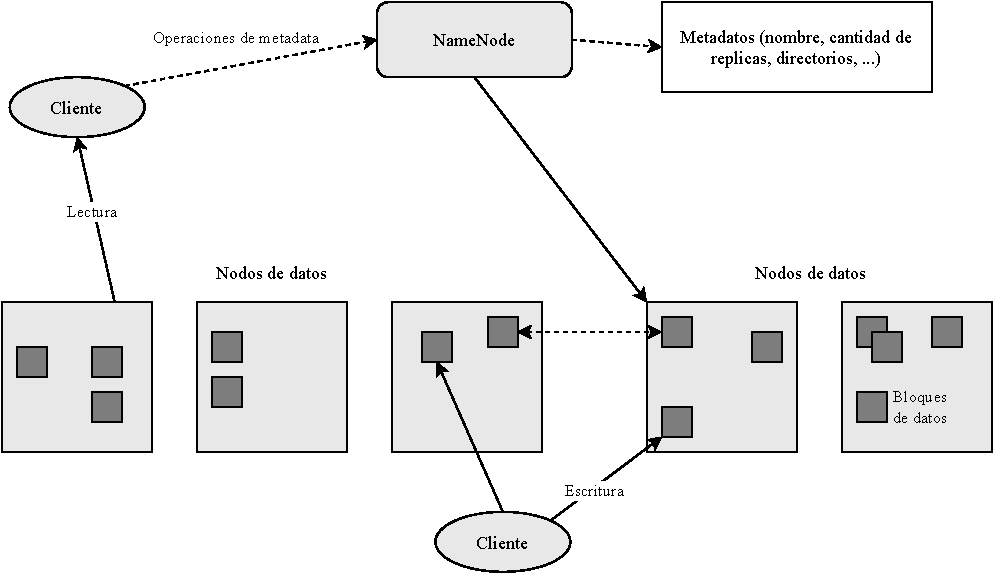
\includegraphics[width=0.9\linewidth]{7_marco_teorico/imagenes/arquitectura_hdfs}
	\caption{Arquitectura HDFS.}
	\label{fig:arquitectura_hdfs}
\end{figure}

\bigskip Tanto el NameNode como el DataNode son piezas de software diseñadas para correr, típicamente, en sistemas operativos GNU/Linux. Además, como HDFS está construido utilizando el lenguaje de programación Java, puede ser desplegado en un rango amplio de máquinas.

\paragraph{Apache Spark}
Apache Spark es una plataforma de código abierto escrita en Scala\footnote{Sitio oficial del lenguaje de programación Scala: https://www.scala-lang.org/. Último acceso: Febrero 2021.}, para procesamiento de datos a gran escala y preparado para tareas de Machine Learning iterativas \citep{meng2016mllib}. En alto nivel, una aplicación Spark consiste en un programa “driver” que ejecuta la función “main” y varias operaciones en paralelo en un cluster de computadoras\footnote{Red de computadoras de alta velocidad que se comportan como si fuesen un único servidor. No confundir con la definición de “cluster” en algoritmos de clustering.}.

\bigskip El paralelismo en un cluster de computadoras realizado por Spark se basa en particiones de datos, por ejemplo, si se desea procesar un conjunto de datos de un millón de registros y se cuenta con un cluster de 4 nodos (sin contar el nodo principal), cada uno de ellos procesará 250.000 registros. Para conseguir esto de una forma que pueda ser entendible para un desarrollador, la plataforma cuenta con una abstracción de datos llamada RDD o \textit{Resilient Distributed Dataset} (o conjunto de datos distribuido resiliente), la cual es una colección de datos particionados a través de los nodos de cluster que pueden operar en paralelo. Los RDDs son creados desde un archivo HDFS o una colección Scala existente en el programa driver. También es posible almacenarlos en memoria, permitiendo que estas colecciones sean reusadas eficientemente entre operaciones paralelas.

\bigskip Los RDDs permiten dos tipos de operaciones: \textit{transformaciones}, las cuales crean un conjunto de datos desde uno existente, y \textit{acciones} u \textit{operaciones terminales}, que devuelven un valor al programa driver luego de ejecutar una cierta cantidad de cómputos en el conjunto de datos. Estas operaciones se condicen con el modelo de programación map-reduce en el cual se basa Hadoop. Por ejemplo, map es una transformación que opera en cada uno de los elementos del conjunto de datos y devuelve un nuevo RDD representando los resultados. Por otro lado, reduce es una operación que agrega todos los elementos de un conjunto de datos usando alguna función y devolviendo un resultado final.

\bigskip Todas las transformaciones son \textit{lazy}, esto es, secuencias de acciones imperativas las cuales son retrasadas hasta que el resultado es requerido \citep{launchbury1993lazy}, es decir, las transformaciones aplicadas a un conjunto de datos son recordadas hasta que es necesario devolver un resultado final al programa driver. Además, es posible almacenar un RDD en memoria (o disco rígido) logrando así mantener elementos disponibles en un cluster para un acceso rápido en caso de que una transformación sea requerida más de una vez.
\subsection{Medidas de distancia de texto}
\subsubsection{Conceptos básicos}
\paragraph{Information retrieval}
\textit{Information retrieval} (IR) se define como encontrar material (generalmente documentos) de una naturaleza desestructurada (generalmente texto) que satisfaga una necesidad de información de grandes colecciones (generalmente almacenadas en computadoras) \citep{schutze2008introduction}.

\bigskip El IR utiliza técnicas probabilísticas, pero también, en los últimos años, investigadores se han centrado en técnicas basadas en conocimiento. Estas últimas, han hecho una significante contribución al IR “inteligente”. Más recientemente, la investigación se ha volcado a nuevas técnicas de aprendizaje inductivo basadas en \textit{inteligencia artificial} (IA), las cuales incluyen redes neuronales, aprendizaje simbólico y algoritmos genéticos \citep{chen1995machine}. Cuando hablamos de aprendizaje, nos referimos a un fenómeno multifacético. Los procesos de aprendizaje incluyen la adquisición de un nuevo conocimiento declarativo, la organización del nuevo conocimiento, representaciones efectivas, y un descubrimiento de nuevos hechos y teorías a través de la observación y la experimentación. Desde el nacimiento de la era de las computadoras, estas capacidades han querido ser implantadas en las mismas. El estudio y el modelado en computadoras del proceso de aprendizaje en múltiples manifestaciones constituyen el propósito principal del Machine Learning \citep{mitchell2013artificial}.

\bigskip Los Sistemas de Recomendación a los cuales se hace foco en este trabajo, aplican técnicas que no son más que conceptos derivados de IR y algunos de ML. Técnicas probabilísticas y determinísticas son utilizadas para extraer información relevante desde diferentes orígenes de datos, así como también generar información valiosa a partir de ellos. Para este último propósito, se han desarrollado métodos basados en el aprendizaje inductivo que demostraron ser muy efectivos y, en algunos casos, fueron útiles para modelos simples y aplicables que permiten desarrollar RSs eficaces y escalables.

\paragraph{Unidad de documento}
Una \textit{unidad de documento}, es una secuencia de caracteres de longitud fija con las cuales se va a trabajar. Estas secuencias de caracteres pueden estar codificadas por uno o varios bytes o esquemas de codificación multibyte, como UTF-8 o varios estándares específicos de algún país o compañía. Una vez que la codificación esté determinada, se debe decodificar la secuencia de bytes a una secuencia de caracteres.

\paragraph{Stopwords}
En informática, se llama stopword a una palabra que se filtra antes o después del procesamiento de datos del lenguaje natural \citep{leskovec2014mining}. Generalmente, este tipo de palabras son extremadamente comunes, y podrían tener poco valor en el momento de seleccionar documentos que coincidan con las necesidades de un usuario \citep{schutze2008introduction}.

\bigskip Entonces, es necesario seleccionar una lista de stopwords, que serán filtradas en el procesamiento de las unidades de documento. Estas listas son llamadas \textit{stop lists}. La estrategia general para el armado de stop lists, es ordenar los términos por \textit{collection frequency}, es decir, el número total de veces que aparece un término en la colección de documentos. Una vez hecho esto, es necesario tomar los términos más frecuentes, a veces filtrados a mano según su contenido semántico relativo al dominio de los documentos que están siendo indexados.

\paragraph{Tokenización}
Dado una secuencia de caracteres y una unidad de documento definida, la \textit{tokenización} es la tarea de dividirla en distintas piezas, llamadas \textit{tokens} y, quizás en el mismo momento, desechar ciertos caracteres (como signos de puntuación). Un ejemplo de tokenización de una secuencia de caracteres en idioma inglés, podría ser:

\begin{verbatim}
Input: Friends, Romans, Countrymen, lend me your ears;
Output: [Friends] [Romans] [Countrymen] [lend] [me] [your] [ears]
\end{verbatim}

Estos tokens, son frecuentemente confundidos con palabras, pero es importante hacer la distinción entre \textit{token}, \textit{tipo}, y \textit{término}, para comprender la diferencia. Un token es una instancia de una secuencia de caracteres en un documento en particular que están agrupados juntos como una unidad semántica útil para procesamiento. Un tipo es la clase de todos los tokens que contienen la misma secuencia de caracteres. Un \textit{término} es un tipo, que es incluido en un diccionario de un sistema de IR. Por ejemplo, si un documento a ser indexado es “to sleep perchance to dream”, existen 5 tokens, pero solo 4 tipos (ya que hay dos instancias del token “to”). Sin embargo, si “to” es desechada por ser un stopword, habrá entonces 3 términos: “sleep”, “perchance” y “dream”.

\paragraph{Similaridad}\label{paragraph:similaridad}
Es de interés poder cuantificar la relación entre los objetos de texto. Existen distintas maneras de medir esa relación. En general se habla de medidas de proximidad \citep{xu2008clustering}. Las medidas de proximidad son una generalización para las medidas de similaridad y disimilaridad. En este trabajo utilizaremos medidas de similaridad comúnmente encontradas en la literatura \citep{resnik1995using, lin1998information, gomaa2013survey, harispe2015semantic}. Debido al propósito de este trabajo, es de interés, en particular, la similaridad semántica en taxonomías \citep{resnik1995using}, que se basa en el contenido de información de las unidades documentales.

\bigskip Las medidas basadas en contenido de información de una unidad de documento (o concepto) en una taxonomía, utilizan el siguiente enfoque.  Se define \(p(t)\) como la probabilidad de un concepto \(t\), formalizando:
\[p(t)=\frac{freq(t)}{N}\]
donde \(freq(t)\) es la frecuencia que aparece un concepto, teniendo en cuenta el concepto en sí y todos sus antecesores; y \(N\) la cantidad total de conceptos en el corpus. De esta forma, el nodo raíz tendrá \(p(t) = 0\), mientras los nodos hojas, tendrán valores cercanos a 1. Se define el contenido de información \(I(t) = 0\) como:
\[I(t)=-\log p(t)\]

Aplicando el logaritmo negativo a \(p(t) = 0\) se logra que los nodos hoja, siendo conceptos muy específicos, contengan mucha información, y que los nodos más genéricos que se encuentran cerca de la raíz posean un contenido de información que, por lo contrario, tienda a cero.

\bigskip \cite{resnik1995using} define, en un conjunto de conceptos \(C\) en una taxonomía \textit{es-un} que permite herencia múltiple, que la similaridad entre dos conceptos es la medida en que ellos comparten información en común, indicado, en este tipo de taxonomías, por el nodo inmediato de más alto nivel que los subsume a ambos, el \textit{subsumidor mínimo} (minimum subsumer o ms por sus siglas en inglés).

\bigskip Considerando dos términos \(t_i\) y \(t_j\), y a \(S(t_i, t_j)\) al conjunto de ancestros comunes de \(t_i\) y \(t_j\), se define al subsumidor mínimo, \(ms(t_i, t_j)\), como al término de \(S(t_i, t_j)\) que contiene el máximo contenido de información:
\[\max_{t \in s(t_i,t_j)} I(t) = I(ms(t_i,t_j))\]

La medida de similaridad de \cite{resnik1995using} \(S_R\), es entonces, el contenido de información del subsumidor mínimo de dos términos:
\[S_R = I(ms(t_i,t_j))\]

El enfoque anterior, posee la siguiente particularidad: no tiene en cuenta la similaridad de los nodos con respecto a su subsumidor mínimo. Es intuitivo pensar que dos conceptos abstractos (nodos ubicados en posiciones más cercanas al subsumidor mínimo) son más parecidos entre sí que dos conceptos específicos (más alejados del subsumidor mínimo) \citep{lin1998information}. Para solucionar esto, \cite{lin1998information} tiene en cuenta dos aspectos para calcular la similaridad entre dos conceptos en este tipo de taxonomías: \begin{enumerate*} [label=(\roman*)] \item La cantidad de información; y \item La ubicación relativa entre los nodos hijos respecto al subsumidor mínimo.\end{enumerate*} Definida como la similaridad de \cite{resnik1995using}.

\bigskip La medida de Lin es:
\[S_L(t_i, t_j)=\frac{2S_R(t_i,t_j)}{I(t_i)+I(t_j)}\]

El resultado de esta medida, estará normalizada en el rango \([0, 1]\) y obtiene que nodos más generales, con menor cantidad de información, sean más similares entre sí, que dos nodos específicos (ya que la cantidad de información de los mismos aumentará el denominador de la ecuación, disminuyendo el resultado final). Se ha demostrado que esta definición de similaridad produce una correlación ligeramente mayor con los juicios humanos.

\paragraph{Medidas de proximidad}
Proximidad es la generalización de similaridad y disimilaridad. La función disimilaridad, también conocida como función de distancia, en un conjunto de datos X, es definida para satisfacer las siguientes condiciones. Las condiciones mencionadas, son las utilizadas por \cite{xu2008clustering} y de relevancia en el presente trabajo:

\begin{enumerate}
	\item Simetría,
	\[D(x_i,x_j)=D(x_j,x_i);\]

	\item Positividad,
	\[D(x_i,x_j) \geq 0 \quad \forall x_i,x_j;\]
\end{enumerate}

De forma, análoga la función de similaridad es definida satisfaciendo las condiciones:
\begin{enumerate}
	\item Simetría,
	\[S(x_i,x_j)=S(x_j,x_i);\]

	\item Positividad,
	\[0 \leq S(x_i,x_j) \leq 1, \quad \forall x_i,x_j\]
\end{enumerate}

Si bien el término matemático de distancia exige una serie de supuestos rigurosos \citep{xu2008clustering}, en este trabajo utilizaremos la noción de distancia y de disimilaridad en forma indistinta, y nos basaremos en las medidas de proximidad habitualmente utilizadas para comparación de texto. Por lo tanto, para transformar una medida de similaridad \(S(x_i,x_j)\) en una de distancia \(D(xi,xj)\) que cumpla \(0 \leq D(x_i,x_j) \leq 1\), haremos la normalización de la misma en el intervalo \([0,1]\) y luego aplicaremos el cálculo \(D(x_i,x_j) = 1 - S(x_i,x_j)\) y recíprocamente \citep{leale2013novel}.

\paragraph{Modelo de espacio vectorial}
En el modelo de espacio vectorial, un texto es representado como un vector de términos. Si las palabras son elegidas como términos, entonces cada palabra del vocabulario sería una dimensión independiente en el espacio vectorial \citep{singhal2001modern}. Todo texto puede ser representado por un vector en este espacio dimensional. Si un término pertenece a un documento, este obtiene un valor distinto de cero en el vector, junto con la dimensión correspondiente al término. Como un documento contiene un conjunto limitado de términos (el vocabulario puede contener millones de términos), muchos de los vectores pueden ser muy dispersos. La mayoría de los sistemas basados en vectores trabajan en el cuadrante positivo, es decir, a ningún término se le asigna un valor negativo.

\bigskip Para asignar un valor numérico a un documento en una consulta, el modelo mide la similaridad entre el vector ingresado en ella y el vector del documento al cual se quiere consultar. La similaridad entre dos vectores no es inherente al modelo. Típicamente, el ángulo entre los dos vectores es usado como medida de divergencia entre los mismos, y el coseno del ángulo es usado como similaridad numérica, ya que el coseno tiene la propiedad de ser tener resultado 1 cuando los vectores son idénticos y 0 cuando los vectores son ortogonales (explicado en detalle más adelante). Como una alternativa, el producto escalar entre dos vectores, es también usado como medida de similaridad. Si todos los vectores están forzados a tener longitud 1, es decir, vectores unitarios, entonces el coseno del ángulo entre los vectores, tiene el mismo resultado que el producto escalar.

\bigskip Formalizando, si \(\overrightarrow{D}\) es el vector del documento y \(\overrightarrow{Q}\) es el vector de la consulta, la similaridad entre \(\overrightarrow{D}\) y \(\overrightarrow{Q}\) es representada como:
\[S(\vec{D},\vec{Q})=\sum_{ti \in Q,D}^{ }{W_{t_{iQ}}.W_{t_{iD}}}\]

donde \(W_{t_{i \overrightarrow{Q}}}\) es el valor de la componente número \(i\) del vector \(\overrightarrow{Q}\) y \(W_{t_{i \overrightarrow{D}}}\) es el valor de la componente número \(i\) del vector \(\overrightarrow{D}\), también definido como el peso del término \(i\) en el documento \(D\). Cualquier término no presente en la consulta o en el documento tendrá valor cero en \(W_{t_{i \overrightarrow{Q}}}\) o \(W_{t_{i \overrightarrow{D}}}\), por lo cual es posible hacer la sumatoria solo de los términos en común entre la consulta y el documento.

\paragraph{Distancia del coseno}
La \textit{distancia del coseno} puede ser la que se aplica en mayor frecuencia en términos de similaridad en IR \citep{korenius2007principal}. Al aplicar la distancia del coseno se obtiene un resultado que se encuentra en el rango \([-1, 1]\). El valor \(-1\) significa que los vectores tienen la misma dirección, pero sentidos opuestos. El valor \(1\), por lo contrario, significa que el ángulo comprendido entre los vectores es cero.

\bigskip Particularmente en IR, es de interés el intervalo \([0, 1]\) ya que todos los componentes de un vector que representa a un documento, son no negativos. De esta interpretación, se deriva la definición de la distancia del coseno, restando la medida del coseno de su máximo valor:
\[d_c(\vec{D}_i, \vec{D}_j) = 1 - cos(\vec{D}_i, \vec{D}_j) = 1 - \frac{{\vec{D}_i}'\vec{D}_j}{\sqrt{{\vec{D}_i}'\vec{D}_i}\sqrt{{\vec{D}_j}'\vec{D}_j}}\]

donde \(i \leq i,j \leq n\). Los símbolos \(\overrightarrow{D_i}\) y \(\overrightarrow{D_j}\) son documentos en forma de vectores y \(d_c\) es la distancia entre ellos.

\bigskip Para simplificar, y teniendo en cuenta que estamos hablando de documentos en forma de vectores, la distancia del coseno se puede derivar de la fórmula del \textit{producto escalar} (producto punto). Siendo \(\overrightarrow{D_i}\) y \(\overrightarrow{D_j}\) dos documentos en forma de vectores, se define el producto escalar entre ellos, como:
\[\vec{D}_i.\vec{D}_j = \left \| \vec{D}_i \right \|.\left \| \vec{D}_j \right \|.cos(\theta)\]

siendo \(\left \|\overrightarrow{D_i}\right \|\) y \(\left \|\overrightarrow{D_j}\right \|\) los módulos de los vectores \(\overrightarrow{D_i}\) y \(\overrightarrow{D_j}\) respectivamente, y $\theta$ el ángulo formado entre ellos. Entonces:
\[cos(\theta) = \frac{\vec{D}_i.\vec{D}_j}{\left \| \vec{D}_i \right \|.\left \| \vec{D}_j \right \|}=\frac{\sum_{i=1}^{n}{{d_i}_i{d_j}_i}}{\sqrt{\sum_{i=1}^{n}{{d_i}_i^{2}}}\sqrt{\sum_{i=1}^{n}{{d_j}_i^{2}}}}\]

Donde \(d_i\) y \(d_j\) son los componentes de los vectores \(\overrightarrow{D_i}\) y \(\overrightarrow{D_j}\) respectivamente.

\subsubsection{Term Frequency}
También conocido en la literatura como \textit{Bag of words} (bolsa de palabras) o simplemente, de sus iniciales, bow. \textit{Term Frequency}, o TF; es una técnica donde el orden exacto de los términos es ignorado, pero se basa en el número de ocurrencia de cada uno de ellos \citep{christopher2008introduction} en un documento. Los términos anteriormente mencionados como referencia a esta técnica, se van a usar indistintamente en este documento.

\bigskip Si comparamos las frases en inglés \textit{“Mary is quicker than John”} y \textit{“John is quicker than Mary”}, desde esta perspectiva (ignorando el orden), son idénticas. Esto conlleva a ciertos problemas desde el punto de vista semántico, ya que, si bien el número de ocurrencia de términos es el mismo, el significado de las frases es opuesto. Las palabras son contadas en una \textit{bolsa}, lo cual difiere de la definición matemática de \textit{conjunto}, que no considera los elementos repetidos. Cada palabra corresponde a una dimensión en el espacio de datos resultante y cada documento corresponde a un vector compuesto por valores no negativos en cada dimensión \citep{huang2008similarity}. Con los documentos representados como vectores, se mide el grado de similaridad de dos documentos como la correlación entre los vectores correspondientes, que puede ser cuantificada como el coseno del ángulo entre ellos. Entonces, es posible obtener la distancia entre dos documentos en forma de vectores \(\overrightarrow{D_1}\) y \(\overrightarrow{D_2}\) aplicando:
\[d(\vec{D}_1, \vec{D}_2) = 1 - \frac{\vec{D}_1 \vec{D}_2}{\left \| \vec{D}_1 \right\| \left \| \vec{D}_2 \right\|}\]

\subsubsection{Term Frequency/Inverse Document Frequency}
Hasta ahora, no se ha mencionado que implicancia tiene la frecuencia de cada término en uno o varios documentos de una colección. Se define \textit{document frequency} \(df_t\) como el número de documentos en una colección que contienen el término \(t\), en contraste con TF que indica que tan frecuentemente aparece un término en un documento dado. El propósito de este indicador, es discriminar a nivel documento para asignar un peso a cada uno de los términos existentes en la colección de documentos \citep{christopher2008introduction}, para lo cual se define \textit{inverse document frequency}, o IDF; un indicador basado en la cantidad de documentos que contienen (o son indexados por) un término en cuestión \citep{robertson2004understanding}. La intuición se basa en que si un término de búsqueda se encuentra en muchos documentos, no es un buen discriminador, y se le debe asignar menor peso que a un término que se encuentra en pocos documentos.

\bigskip Este método, conocido como \textit{Term Frequency/Inverse Document Frequency} (TF-IDF), está basado en multiplicar la medida IDF con la medida TF. Asumiendo que existen \(N\) documentos en una colección, y un término \(t_i\) aparece en \(n_i\) documentos (\(df_t\)), entonces la medida IDF propuesta es \citep{sparck1972statistical}:
\[idf(t_i) = \log{\frac{N}{n_i}}\]

Palabras con alto valor TF-IDF implican una fuerte relación con el documento en el cual aparecen, es decir, que TF-IDF mide la relevancia de un término en un documento dado. Estas palabras, que son comunes solo en un documento o en un pequeño grupo de ellos, tienden a tener un valor TF-IDF más grande que palabras comunes como artículos y preposiciones \citep{ramos2003using}.

\bigskip El procedimiento formal para implementar TF-IDF tiene algunas diferencias menores entre diferentes aplicaciones, pero básicamente consiste como se indica a continuación. Siendo \(t_i\) un término que se encuentra en un documento \(d_j\), se calcula:
\[tfidf(t_i, d_j) = tf(t_i, d_j) \cdot idf(t_j)\]
\[tfidf(t_i, d_j) = tf(t_i, d_j) \cdot \log{\frac{N}{n_j}}\]

Esta fórmula deriva en distintos valores que puede tomar el resultado final. Teniendo en cuenta cada uno de los parámetros involucrados, se van a analizar algunas variaciones. Consideremos en principio que \(N \cong n_j\), es decir que el término \(t_i\) aparece en casi todos los documentos. Esto implica que \(1 <  \log(\frac{N}{n_j}) < c \) para un \(c\) con un valor pequeño y el valor de TF-IDF será menor que el valor de IDF, pero aún positivo (ya que \(0 \leq tf(t_i,d_j) \leq 1\)). Esto implica que el término \(t_i\) es relativamente común entre todos los documentos pero aún posee cierta importancia sobre \(N\). Este puede ser el caso de palabras muy comunes en documentos, como pronombres o preposiciones, las cuales no tienen ningún significado relevante por sí mismas, y recibirán un valor TF-IDF muy bajo. Finalmente, supongamos que el valor TF es alto, y \(n_j\) es un número pequeño. Entonces \(\log(\frac{N}{n_j})\) será bastante grande y así también lo será el valor total TF-IDF. Este último caso es en el cual estamos interesados, ya que las palabras con alto TF-IDF implica que son importantes en \(n_j\) pero no son comunes en la totalidad de los documentos. Este término \(t_i\) se dice que tiene un gran \textit{poder discriminatorio}.

\bigskip TF-IDF es un algoritmo eficiente y simple para medir el peso que tiene una palabra en una consulta para un conjunto de documentos que son relevantes para esa consulta. Además, TF-IDF es simple de codificar, sentando las bases para algoritmos más complicados y sistemas de IR. Más allá de esas fortalezas, TF-IDF tiene sus limitaciones. En cuanto a sinónimos, no hace ninguna relación entre palabras. Es decir, que no considerará documentos en los cuales la palabra no se encuentra pero si se encuentra un sinónimo de la misma, ya que las palabras son tomadas como conceptos totalmente diferentes. El mismo problema ocurre cuando se trata de plurales o una variación del tiempo verbal de una palabra, por ejemplo, “país” y “países” serán categorizadas separadas, en lugar de categorizarlas como una sola palabra y calcular un valor TF-IDF más bajo.

\subsubsection{Word2Vec}
\textit{Word2Vec} (W2V) presenta dos modelos basados en redes neuronales para computar representaciones de palabras como vectores continuos en grandes conjuntos de datos. La calidad de la representación es medida como similaridad \citep{mikolov2013efficient}. La forma de representar los vectores está basada en su contexto, el cual es usado para optimizar la representación del vector, es decir, palabras con significado similar son representadas con vectores que están más cerca unos de otros. Esto indica que, por primera vez en las medidas analizadas en el estado del arte de este trabajo, W2V toma un enfoque semántico.

\paragraph{Motivación de Word2Vec}
Muchos sistemas de \textit{procesamiento de lenguaje natural} (NLP por sus siglas en inglés correspondientes a Natural Language Processing), tratan a las palabras o unidades atómicas y no tienen noción de similaridad entre las palabras. Este tipo de sistemas son limitados para varias tareas, ya que no proporcionan información sobre las relaciones que pueden existir entre las distintas entidades. Con el progreso del Machine Learning en los últimos años, ha sido posible entrenar modelos más complejos con grandes conjuntos de datos, y en ellos se observa un rendimiento mejor que en los modelos más simples. Probablemente, el concepto más exitoso es la \textit{representación distribuida de palabras}. En estos modelos, fue descubierto que la similaridad entre palabras va más allá que simples regularidades sintácticas, por el contrario es posible realizar operaciones algebraicas entre representaciones vectoriales de palabras, tal como:

\begin{verbatim}
vector("Rey") - vector("Hombre") + vector("mujer") = vector("Reina")
\end{verbatim}

Los vectores adhieren muy bien a nuestra intuición, por ejemplo, palabras que son sinónimos tienden a tener vectores similares en términos de la distancia del coseno, mientras que antónimos, tienden a tener vectores disímiles. Por lo cual, el objetivo es maximizar la precisión de estas operaciones entre vectores mediante un arquitecturas de modelos que preserven regularidades lineales entre palabras así como también minimizar la complejidad computacional. Estos vectores son útiles por dos razones principales \citep{mccormick2016word2vec}:

\begin{enumerate}
	\item Se puede medir la similaridad semántica entre dos palabras calculando la distancia del coseno entre los vectores correspondientes.
	\item Es posible usar los vectores en distintas tareas de NLP, tales como clasificación de documentos o análisis de sentimientos.
\end{enumerate}

\bigskip Las arquitecturas propuestas por W2V se basan en dos modelos, \textit{Skip-Gram} y \textit{CBOW} (Continuous Bag of Words). Ambos modelos son simples redes neuronales con una capa oculta, y los vectores son resultados de propagación hacia atrás y \textit{descenso de gradiente estocástico} (SDG por sus siglas en inglés correspondientes a Stochastic Gradient Descent). La Figura \ref{fig:cbowskipgram} muestra la diferencia entre ambos modelos, los dos utilizando una capa oculta: a la izquierda, CBOW utiliza un conjunto de palabras y predice la palabra actual \(w(t)\); a la derecha, Skip-gram predice palabras vecinas a partir de una palabra \(w(t)\). El detalle de cada uno de los métodos es descrito a continuación.

\begin{figure}[h!]
	\centering
	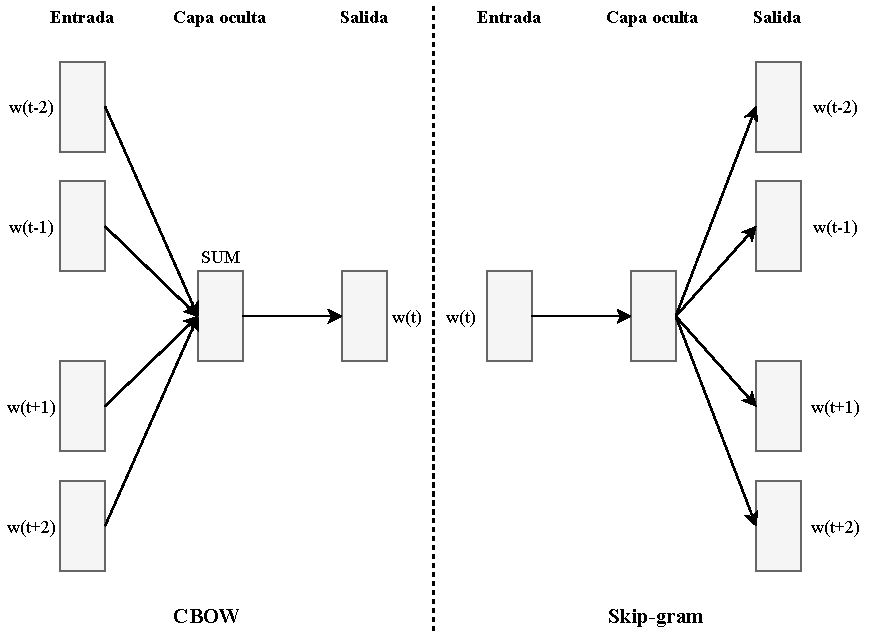
\includegraphics[width=0.7\linewidth]{7_marco_teorico/imagenes/cbow_skipgram.pdf}
	\caption{La arquitectura CBOW predice la palabra actual basándose en el contexto, mientras que la arquitectura Skip-gram predice palabras vecinas, dada una palabra como entrada \citep{mikolov2013efficient}.}
	\label{fig:cbowskipgram}
\end{figure}

\paragraph{Modelo Skip-Gram}
El modelo Skip-gram se basa en lo siguiente: dado un conjunto de frases (llamado \textit{corpus}) el modelo analiza las palabras de cada sentencia y utiliza cada palabra para predecir las palabras que serán vecinas, esta técnica se basa en la \textit{propagación hacia atrás}. La entrada para este modelo es una sola palabra \(w_I\) y la salida, su contexto \(\{w_{0,1},..., w_{0,C}\}\) definido por una ventana de tamaño \(C\). Una potencial instancia de entrenamiento podría ser la palabra “auto” como entrada y las palabras \{"Manejé","mi","hacia","la","tienda"\} las salidas. El objetivo es, mediante el entrenamiento, generar los pesos de la capa oculta de la red neuronal y usarlos como los vectores que representarán las palabras. Mediante la palabra que es usada como entrada, el modelo busca palabras “vecinas” pertenecientes a su contexto y elige una de forma aleatoria. La red neuronal dará como resultado la probabilidad de cada palabra en nuestro vocabulario de ser \textit{palabra vecina}. El concepto de palabra vecina, viene dado por el tamaño de ventana que hayamos elegido, si el tamaño de ventana es 5, significa que son tomadas en cuenta 5 palabras adelante y 5 palabras atrás (10 en total) \citep{skipgrammodel}.

\bigskip La entrada de la red neuronal será una palabra representada como \textit{one-hot vector}, un vector con tantas posiciones como tamaño tenga el vocabulario; esto es, si tenemos un vocabulario de 10000 palabras, el vector tendrá el valor 1 en la posición donde se encuentre la palabra representada, y 0 en las 9999 restantes. La salida de la red neuronal, es otro vector con las mismas 10000 posiciones, que en cada posición contiene las probabilidades de que cada una de las palabras sean vecinas de la palabra representada en la entrada. Las probabilidades son calculadas de la siguiente forma. Dado un one-hot vector \(x\) de tamaño \(V\) (cantidad de palabras del vocabulario) correspondiente a la palabra de entrada, y un conjunto de redes neuronales de la capa oculta de tamaño \(N\). Dado una ventana de tamaño \(C\), tendrémos \(\{y_1,...,y_C\}\) vectores one-hot correspondientes a las palabras de salida en la instancia de entrenamiento. La matriz \(W=V \times N\) es la matriz de pesos entre la capa de entrada y la capa oculta, cuya fila \(i^{th}\) representa los pesos correspondientes a la palabra \(i^{th}\) del vocabulario. Esta matriz \(W\) contiene entonces, la codificación como vector de cada una de las palabras del vocabulario (como filas), las cuales serán entrenadas mediante la red neuronal. El siguiente ejemplo ilustra, cómo la matriz \(W\) multiplicada por el vector de entrada, resulta en el vector que la representa.
\[\begin{bmatrix}0 & 0 & 0 & 1 & 0 \end{bmatrix} \times  \begin{bmatrix}12 & 14 & 2 \\ 6 & 19 & 74 \\ 22 & 33 & 96 \\ 36 & 85 & 2 \\ 95 & 1 & 56 \end{bmatrix} = \begin{bmatrix} 36 & 85 & 2 \end{bmatrix}\]

Se puede ver, cómo el vector resultado de tamaño \(1 \times N\) es la 4 fila de la matriz \(W\), ya que la palabra de entrada es un vector one-hot con el valor \(1\) en el cuarto elemento.

\bigskip Una vez obtenido el vector de salida, éste es usado como entrada para la capa de salida de la red neuronal, usando un clasificador de regresión Softmax \citep{morin2005hierarchical}, el cual es una generalización de la regresión logística para el caso en que se quieren manejar múltiples clases\footnote{Tutorial en profundidad de regresión Softmax \url{http://ufldl.stanford.edu/tutorial/supervised/SoftmaxRegression},  Último acceso: Febrero 2021.}. Cada una de las \(V\) neuronas de la capa de salida, producirá un valor entre \(0\) y \(1\). Además, la suma de todos estos valores, será \(1\), es decir, una distribución de probabilidades. Específicamente, cada neurona de salida tiene un vector de pesos correspondiente a cada una de las palabras del vocabulario, que se multiplica con el vector que proviene de la capa oculta y se aplica una función Softmax. El resultado es la probabilidad de que aleatoriamente se seleccione la palabra de entrada y sea vecina a cada una de las palabras representadas por los vectores en las neuronas de salida.

\paragraph{Modelo Continuous Bag of Works (CBOW)}
Es similar al modelo Skip-gram pero con las salidas y las entradas invertidas: dado un conjunto de palabras que definen un contexto, CBOW predice la palabra actual. La capa de entrada consiste en \(C\) palabras del contexto, codificadas como vectores one-hot, es decir un conjunto \( \{x_1,..., x_C\}\) cada uno de dimensión \(V\). La capa oculta es un vector \(h\) de tamaño \(N\). Finalmente, la salida es una palabra \(y\) también codificada como un vector one-hot. Los vectores de entrada son conectados con la capa oculta por una matriz \(W=V \times N\), y esta capa oculta a su vez es conectada con la capa de salida vía otra matriz \(W'=V \times N\) \citep{cbowmodel}.

\bigskip La salida de la capa oculta \(h\) de la red neuronal es el promedio de los vectores de entrada, ponderados por la matriz \(W\).
\[h = \frac{1}{C}W \cdot (\sum_{i=1}^{C}{x_i})\]
Este cómputo es una de las diferencias principales con el modelo Skip-gram. Luego, se calculan las entradas de cada nodo de la capa de salida.
\[u_j = {v'_{w_j}}^{T} \cdot h\]
donde \(v'_{w_j}\) es la \(j^{th}\) columna de la matriz \(W'\). Y finalmente se calcula el resultado de la capa de salida. Dicha salida \(y_j\) es obtenida pasando la entrada \(u_j\) por la función Softmax.
\[y_j=p(w_{y_j}|w_1,...,w_C)=\frac{exp(u_j))}{\sum_{V}^{j=1}exp(u_j')}\]

\bigskip Entonces, la capa de salida es una palabra \(y_j\) codificada como un vector one-hot de dimensión \(V\).

\subsubsection{FastText}
Fastext\footnote{Sitio de FastText \url{https://fasttext.cc}. Último acceso: Febrero 2021.} es una librería open-source que permite generar representaciones de texto y clasificadores de texto. Está basada en una técnica representación continua de palabras, que tiene en cuenta la morfología\footnote{Parte de la lingüística que estudia las reglas que rigen la flexión, la composición y la derivación de las palabras. Por ejemplo, las distintas conjugaciones de los verbos en español.} de las mismas \citep{bojanowski2017enriching}.
El modelo de FastText está basado en el modelo Skip-gram, donde cada palabra es representada como una bolsa de caracteres \(n-gramas\). Y a cada uno de los n-gramas, se le asignará un vector, que luego, sumados, representarán cada palabra. Dos características muy importantes son, \begin{enumerate*} [label=(\roman*)] \item el método es muy rápido, permitiendo entrenar grandes conjuntos de datos; y \item permite calcular representación de palabras que no aparecen en el conjunto de entrenamiento.  \end{enumerate*}

\bigskip Repasando el modelo Skip-gram, introducido por \cite{mikolov2013efficient}, dado un vocabulario \(V\), donde una palabra es identificada por su índice \(w \in \{1,... , V\}\) , el objetivos es aprender la representación vectorial de cada palabra \(w\). Dado un documento grande representado como una secuencia de palabras \(w_1, ..., w_t\), el objetivo del modelo Skip-gram es que las representaciones de las palabras sean entrenadas para \textit{predecir bien} otras palabras que aparecen en el contexto, es decir, minimizar la siguiente probabilidad logarítmica:
\[\sum_{t=1}^{T}\sum_{c \in C_t}^{T}{\log p(w_c | w_t)}\]
donde el contexto \(C_t\) es el conjunto de índices de palabras que están alrededor de \(w_t\).

\paragraph{Modelo sub-palabra}
Usando una representación en forma de vector para cada palabra, se ignora la estructura interna de las mismas. El modelo sub-palabra, propone una función de scoring \(s\), con el objetivo de tener en cuenta esta información.
Cada palabra \(w\) es representada como una bolsa de n-gramas. Se agregan los símbolos ``\(<\)'' y ``\(>\)'' para delimitar el principio y el final de cada palabra. También, se incluye la palabra en sí misma como otro n-grama. Por ejemplo, la palabra ``where'' y con un \(n = 3\) (longitud de la sub-palabras, en este caso sería, tri-gramas), obtenemos:

\begin{center}\ttfamily\sbox{0}{a}%
	\begin{minipage}{45\wd0}% 45 characters here
		\begin{verbatim}
		'<wh', 'whe', 'her', 'ere', 're>' y '<where>'
		\end{verbatim}
	\end{minipage}
\end{center}

Cabe aclarar que los símbolos ``\(<\)'' y ``\(>\)'' también son considerados como caracteres a la hora de construir los n-gramas. Por ejemplo, ``\(<wh\)'' es un trigrama con un delimitador de inicio de palabra.

\bigskip Dado un diccionario de n-gramas de tamaño \(G\) y una palabra \(w\), el conjunto de n-gramas que aparecen en \(w\) es \(G_w \in \{1,..., G\}\). Se asocia un vector \(z_g\) a cada n-grama \(g\). Se representa una palabra, como la suma de todas las representaciones vectoriales de sus n-gramas. Entonces, la función scoring, es:
\[s(w,c) = \sum_{g \in G_w}^{}{}z_g^T v_c\]

Este modelo, permite compartir las representaciones entre las palabras y, también, aprender una representación confiable de palabras extrañas o poco frecuentes.

\subsubsection{Semantic Distance}
La \textit{distancia semántica} usada en este trabajo está basada en redes semánticas y estadísticas de corpus \citep{li2006sentence}. El método en cuestión está basado en el cálculo de similaridad entre textos de distancia corta, que tiene en cuenta la información semántica y la información del orden de las palabras implicadas en las frases involucradas. La información semántica de las frases es obtenida desde una base de datos léxica y \textit{estadísticas de corpus}\footnote{El estudio de los aspectos estadísticos de los textos se ha centrado tradicionalmente en el análisis de la frecuencia de los elementos y fenómenos que se encuentran en ellos, especialmente en lo referido al componente léxico.}. El uso de una base de datos léxica posibilita modelar el sentido común humano y las estadísticas de corpus adaptar el método a diferentes dominios.

\bigskip Uno de los puntos dominantes por el cual este método es particularmente efectivo para calcular similaridad entre frases cortas se basa en que, tradicionalmente los métodos basados en palabras comunes funcionan bien solo para textos largos, para los cuales existe una alta posibilidad de que una palabra se encuentre en los documentos en comparación. En cambio, para textos cortos, la coocurrencia de palabras entre ellos es muy rara o nula. Esto se debe a la flexibilidad de los lenguajes de expresar mismos significados usando diferentes frases en términos de estructura y palabras.

\paragraph{El método}
\begin{figure}[h!]
	\centering
	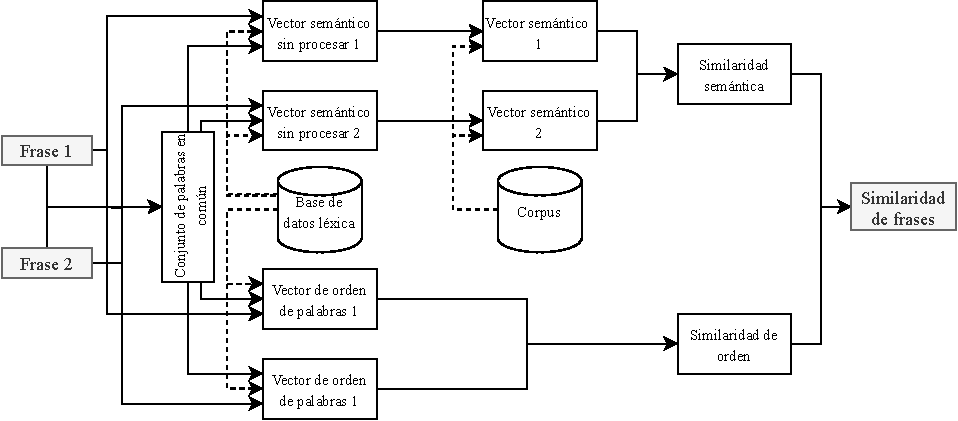
\includegraphics[width=0.9\linewidth]{7_marco_teorico/imagenes/similaridad_sematinca_metodo}
	\caption{Diagrama de cálculo de similaridad semántica.}
	\label{fig:similaridadsematincametodo}
\end{figure}

El procedimiento de cálculo de similaridad entre dos frases, como se muestra en la Figura \ref{fig:similaridadsematincametodo}, utiliza un conjunto de palabras en común usando todas las palabras distintas en el par de frases (en lugar de usar un conjunto fijo como vocabulario). De cada una de las frases, un vector semántico sin procesar es derivado, utilizando la base de datos léxica. También, un vector de orden de palabras es generado a partir de cada frase utilizando la base de datos. Como cada palabra en una frase, contribuye de forma diferente al significado de la misma, la importancia de cada una de ellas es ponderada utilizando información de contenido derivado del corpus. Combinando la información de corpus con los vectores semánticos sin procesar, se obtienen nuevos vectores semánticos los cuales servirán para calcular la \textit{similaridad semántica}. Una \textit{similaridad de orden} es calculada usando los dos vectores de orden previamente generados. Finalmente, la similaridad entre frases es calculada combinando la similaridad semántica y la similaridad de orden.

\paragraph{Similaridad semántica entre palabras}
Las bases de conocimiento tienden a representar el sentido común humano con una estructura jerárquica para un dominio específico o para un lenguaje en general. Existen varios proyectos lingüísticos disponibles en la web, tales como WordNet \citep{miller1995wordnet}, Spatial Date Transfer Standard de la USGS\footnote{United States Geological Survey. https://www.usgs.gov/. Último acceso: Febrero 2021.}, y Gene Ontology\footnote{Gene Ontology. http://geneontology.org/. Último acceso: Febrero 2021.}. Esta estructura jerárquica, se puede modelar como una taxonomía de conceptos.

\bigskip Dadas dos palabras \(w_1\) y \(w_2\), es necesario encontrar la similaridad \(S(w_1,w_2)\) entre ellas. Esto es posible analizando la base de datos léxica (en este caso WordNet si se cuenta con palabras en el idioma inglés) de la siguiente forma: Las palabras están organizadas como conjuntos de sinónimos (llamados \textit{synsets}), con relaciones semánticas a otros synsets. Un método directo para calcular la similaridad es encontrar el camino más corto que conecta dos palabras. Por ejemplo, si tomamos la estructura detallada en la Figura \ref{fig:taxonomiasemantica}, la cual muestra un esquema de base de datos semántica en forma jerárquica que tiene como raíz al synset ``entidad'', el camino más corto para conectar ``niño'' y ``niña'' sería ``niño-persona masculina-humano-persona femenina-niña'', y tiene una longitud de \(4\). El synset ``persona, humano'', en este caso, es llamado \textit{subsumidor mínimo de palabras}, tal como se menciona en la sección \ref{paragraph:similaridad}, ya que sirve de anclaje entre los dos conceptos para los cuales se quiere calcular la distancia semántica.

\begin{figure}[h!]
	\centering
	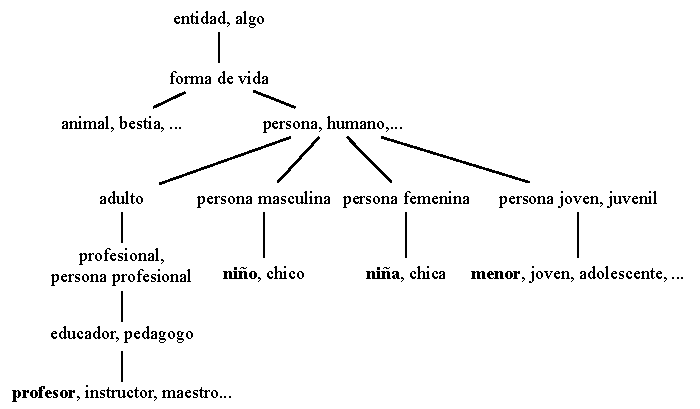
\includegraphics[width=0.9\linewidth]{7_marco_teorico/imagenes/taxonomia_semantica}
	\caption{Base de datos semántica de forma jerárquica.}
	\label{fig:taxonomiasemantica}
\end{figure}

También, se puede ver que la distancia entre ``niño'' y ``profesor'' es 6, mientras la distancia entre ``niño'' y ``animal'' es 4, lo cual es contra intuitivo e indica que el proceso es mejorable agregando más información de estas estructuras jerárquicas. Es evidente que los synsets pertenecientes a capas altas de la estructura tienen conceptos semánticos más generales y menos similaridad entre ellos, y en capas inferiores, sucede lo contrario, conceptos más particulares y similares. Lo anterior sugiere tomar en cuenta la profundidad en jerarquía. Para resumir, la similaridad entre palabras es determinada, no solo por el camino más corto entre ellas, sino también por la profundidad jerárquica, es decir:
\[S(w_1,w_2)=f(l,h)\]

donde \(l\) es el camino más corto entre \(w_1\) y \(w_2\), y \(h\) es la profundidad del subsumer de las mismas en la jerarquía de la red semántica.

\paragraph{Similaridad semántica entre frases}
Contrariamente a métodos clásicos que usan vocabularios con miles de palabras precompiladas, este método semántico usa únicamente vectores semánticos formados por las frases en comparación. Un conjunto de palabras comunes \(T\) es formado por la unión de las dos frases en comparación, luego, un vector semántico léxico es derivado. Cada entrada del vector corresponde a una palabra del conjunto de palabras comunes, lo cual indica que la dimensión del vector es igual al número de palabras del conjunto. El valor de una entrada del vector semántico es calculado de la siguiente forma:
\begin{itemize}
	\item \textbf{Caso 1}.  Si \(w_i\) aparece en la frase, \(s_i\) es 1.
	\item \textbf{Caso 2}. Si \(w_i\)  no está contenida en \(T_1\), una similaridad semántica es calculada entre \(w_1\) y cada palabra en \(T_1\) utilizando el método de la sección anterior.
\end{itemize}

Luego, es necesario ponderar cada una de las palabras basadas en su contenido de información \citep{ribadas2005semantic}. Cada celda es ponderada por la información de contenido \(I(w_i)\) y \(I(\widetilde{w}_i)\). Finalmente, el valor de la entrada del vector semántico es:
\[s_i = \check{s} \cdot I(w_i) \cdot I(\widetilde{w}_i)\]

donde \(w_i\) es una palabra en el conjunto de palabras comunes, y \(I(\widetilde{w}_i)\) es su palabra asociada en la frase. Entonces, la similaridad semántica entre dos frases es definida como el coeficiente del coseno entre los dos vectores:
\[S_s = \frac{s_1. s_2}{||s_1||.||s_2||}\]

\paragraph{Similaridad de orden entre frases}
Consideremos dos frases \(T_1\) y \(T_2\), por ejemplo:
\begin{itemize}
	\item \textbf{T1}:  A quick brown dog jumps over the lazy fox.
	\item \textbf{T2}. A quick brown fox jumps over the lazy dog.
\end{itemize}

Estas frases tienen exactamente las mismas palabras, pero dos de ellas, ubicadas en orden inverso. Como las dos frases contienen las mismas palabras, un método basado en Bag of Words, resultará en que las frases son idénticas, pero para un intérprete humano, es claro que las frases sólo son similares en cierto grado. Por lo cual, un método computacional de similaridad entre frases debe tener en cuenta el orden de las palabras. En el ejemplo, el conjunto de palabras comunes es:

\begin{center}\ttfamily\sbox{0}{a}%
\begin{minipage}{45\wd0}% 45 characters here
	\begin{verbatim}
T = {A quick brown dog jumps over the lazy fox}
	\end{verbatim}
\end{minipage}
\end{center}

Para lograr esto, este método asigna un índice único por cada palabra en \(T_1\) y \(T_2\), en orden, armando un arreglo de palabras. Un vector de orden \(r\) es formado para \(T_1\) y \(T_2\), respectivamente, basado en el conjunto de palabras comunes. Tomando \(T_1\) como ejemplo, por cada palabra \(w_i\) en \(T\), se intenta encontrar la palabra más similar en \(T_1\) de la siguiente forma:
\begin{enumerate}
	\item Si la misma palabra está presente en \(T_1\), la entrada por la palabra en \(r_1\) será el índice de la misma en \(T_1\). Caso contrario, se intenta buscar la palabra más similar \(\widetilde{w}_i \) semánticamente.
	\item Si la similaridad entre \(w_i\) y \(\widetilde{w}_i \) es mayor al umbral, la entrada de \(w_i\) en \(r_1\) es completada con el índice de \(\widetilde{w}_i \) en \(T_1\).
	\item Si las dos búsquedas anteriores fallan, la entrada de \(w_i \) en \(r_1\) es \(0\).
\end{enumerate}
Aplicando este procedimiento a las frases de ejemplo, tenemos:
\[r_1 = \left \{\;1\;2\;3\;4\;5\;6\;7\;8\;9\;\right \}\]
\[r_2 = \left \{\;1\;2\;3\;9\;5\;6\;7\;8\;4\;\right \}\]
Se propone una medida de similaridad de orden entre frases como:
\[S_r = 1 - \frac{\left \| r_1 - r_2 \right \|}{\left \| r_1 + r_2 \right \|}\]
Esto significa que la similaridad de orden de palabras es determinada por la diferencia normalizada del orden de palabras.

\paragraph{Similaridad total entre frases}
La similaridad semántica y la información sintáctica (en términos del orden de las palabras) convergen en el significado de la oración. Entonces, la similaridad total entre frases es definida como la combinación de la similaridad semántica y la similaridad del orden de palabras:
\[S(T_1, T_2)=\delta S_s + (1 - \delta)S_r\]
\[S(T_1, T_2)=\delta \frac{s_1.s_2}{\left \| s_1 \right \|\left \| s_2 \right \|} + (1 - \delta)\frac{\left \|r_1-r_2  \right \|}{\left \| r_1+r_2 \right \|}\]

\bigskip donde \(\delta \leq 1\) decide la contribución relativa de cada una de las medidas de similaridad. Como el orden de palabras cumple un rol subordinado, se recomienda que \(\delta\) tenga un valor mayor a \(0.5\).


\subsection{Ensamble de Clustering}
\subsubsection{Clustering}\label{sec:clustering}
El Clustering o \textit{análisis cluster} tiene por objetivo agrupar elementos en grupos homogéneos en función de las similitudes o similaridades entre ellos. Normalmente se agrupan las observaciones, pero el Clustering puede también aplicarse para agrupar variables. Estos métodos se conocen también con el nombre de \textit{métodos de clasificación automática o no supervisada}, o de reconocimiento de patrones sin supervisión \citep{pena2013analisis}. Con esta información de clasificación a mano, se puede inferir las propiedades de un objeto específico, basándose en la categoría que pertenece. Básicamente, los sistemas de clasificación son supervisados o no supervisados, dependiendo si asignan nuevos objetos de datos a uno o a un número finito de clases supervisadas discretas o categorías no supervisadas, respectivamente \citep{xu2008clustering}.

\paragraph{Definición de Cluster}
Los algoritmos de clustering agrupan objetos de datos (patrones, entidades, instancias, observaciones, unidades) en un cierto número de clusters (grupos, subconjuntos o categorías).

\bigskip En \citep{everittcluster} se presenta la siguiente definición: “un cluster es un conjunto de entidades que son similares, y entidades de clusters diferentes no son similares”. Claramente, esta similaridad y disimilaridad debe ser definida con un criterio significativo, tales como las medidas de proximidad comentadas anteriormente.

\paragraph{Algoritmos de Clustering}\label{sec:algoritmos_clustering}
Los algoritmos de clustering están generalmente clasificados en \textit{clustering particional} y \textit{clustering jerárquico}, basándose en la forma que se generan los clusters \citep{xu2008clustering}. Los algoritmos de clustering jerárquico encuentran clusters anidados recursivamente en un modo aglomerativo, esto es, empezando con cada uno de los puntos de datos como si fueran clusters y combinándolos con el más similar, sucesivamente, para formar de este modo una jerarquía de clusters; o bien en modo divisivo (de arriba hacia abajo --en inglés, top-down--), esto es, empezando con todos los puntos de datos en un cluster y dividiendo recursivamente cada uno de los clusters en clusters más pequeños. Los algoritmos de clustering particional intentan encontrar todos los clusters simultáneamente como una partición de datos, y no imponen una estructura jerárquica; la base matemática es simple: se parte del concepto de \textit{partición}, donde no existen subconjuntos solapados y la unión de los subconjuntos es exactamente el conjunto total. La entrada de un algoritmo jerárquico es una matriz de similaridad \(n \times n\) , donde \(n\) es el número de objetos a ser analizados por medio de clustering. Por otro lado, los algoritmos particionales puede usar tanto una matriz \(n \times d\), representando \(n\) objetos en un espacio d-dimensional, o bien, como un algoritmo jerárquico, una matriz \(n \times n\) \citep{jain2010data}.

\bigskip En este trabajo, nos centraremos en algoritmos particionales, utilizando medidas de proximidad de texto para determinar cuáles objetos (cadenas de texto) pertenecerán al mismo cluster y cuáles no. Algunos ejemplos de este tipo de algoritmo son el ampliamente utilizado \textit{k-medias} \citep{macqueen1967some}, y también el \textit{Particionamiento Alrededor de Medoids (PAM)} o \textit{k-medoids}. Este último se utilizará en este trabajo, por lo cual es descrito a continuación.

\paragraph{Particionamiento Alrededor de Medoides (PAM)}
Particionamiento Alrededor de Medoides (PAM) es un algoritmo de Clustering particional, cuyo funcionamiento es similar al del k-medias, pero en lugar de tomar un conjunto de datos aleatorio como centroides y luego, iterativamente, calcularlo como medias de los clusters, se utilizan puntos, llamados \textit{medoides}, “representativos” de un cluster, y tienen la particularidad de estar más céntricamente ubicados en el mismo \citep{rdusseeun1987clustering}. A diferencia de los centroides del algoritmo k-medias, que son vectores que pueden tomar valores arbitrarios en el espacio d-dimensional de elementos de entrada, los medoides son puntos que representan a un subconjunto de los mismos elementos. En este caso no se trabaja con otros datos fuera del conjunto de datos de entrada.

\bigskip PAM tiene dos etapas, denominadas BUILD (construcción, etapa de formación de los clusters) y SWAP (intercambio, etapa de refinamiento de la partición obtenida). Nos centraremos en la etapa BUILD, ya que será la utilizada en este trabajo:
\begin{enumerate}
	\item Establecer el medoide inicial \(m_1\) como el vector de características del conjunto de datos de entrada que minimiza la distancia a todos los demás datos en \(X\).
\[m_1 = arg \> \underset{\forall x_i}{min} \sum_{j \neq i}d(x_i,x_j),\]
donde \(d(x_i,x_j)\) es una medida de distancia genérica.
	\item Considerar un vector previamente no seleccionado \(x_i\).
	\item Considerar un vector previamente no seleccionado \(x_j\) y calcular la diferencia entre su distancia al medoide previamente seleccionado \(m_1\), y su distancia al vector \(x_i\).
	\item Calcular la Contribución \(C(x_i,x_j)\) del vector \(x_j\) a la selección del vector \(x_i\), como:
\[C(x_i, x_j) = max(d(x_j, m_1) - d(x_j, x_i), 0).\]
	\item Calcular la Ganancia total obtenida a partir de la selección del vector \(x_i\) como:
\[G(x_i) = \sum_{j} C(x_j, x_i).\]
	\item Establecer el siguiente medoide como el vector previamente no seleccionado que maximiza la ganancia total, esto es:
\[m_l = arg \> \underset{\forall i}{max} \> G(x_i).\]
	\item Repetir los pasos 2 al 6 hasta llegar a obtener \(k\) medoides.
\end{enumerate}

\bigskip El método PAM puede aceptar una matriz de distancias como entrada, lo cual lo hace adecuado para utilizar las salidas de los métodos anteriormente mencionados. Como desventaja, se puede mencionar que su complejidad temporal es cuadrática, lo que se traduce como poca eficiencia en grandes conjuntos de datos, sin embargo, se han desarrollado mejoras sobre PAM para estos problemas de desempeño \citep{kaufman2009finding}.

\subsubsection{Ensamble de clustering}
Distintos algoritmos de clustering producen distintos grupos de objetos, en forma de particiones de datos. Incluso el mismo algoritmo con distintos parámetros también produce distintos grupos de datos de salida \citep{xu2008clustering}. Además, las combinaciones de diferentes representaciones de datos que no pueden ser localizadas en un espacio dimensional, pueden generar particiones de datos completamente diferentes. El Ensamble de Clustering, propone un método para extraer clusters consistentes dadas particiones variadas de entrada.

\bigskip Dado un conjunto de datos de \(n\) objetos o patrones y \(d\) dimensiones, se aplican distintas técnicas de clustering a los mismos. Luego, usando Clustering de Acumulación de Evidencias (EAC), cada partición es vista como una evidencia independiente de organización de datos, las cuales se combinan, generando una nueva matriz de similaridad \(n \times n\) entre los \(n\) patrones. Esta matriz poseerá una similaridad para cada par de elementos que será tanto más grande cuanto más veces dichos elementos participen en el mismo cluster para las sucesivas evidencias encontradas. La partición de datos final entre los \(n\) patrones es obtenida aplicando un algoritmo de clustering en la matriz de similaridad \citep{fred2005combining}.

\bigskip Debido a la existencia de muchos algoritmos de clustering, y a la posibilidad de poder variar los mismos con distintos parámetros de entrada, es difícil encontrar un algoritmo o variación del mismo que produzca los resultados esperados, funcione con distintas formas de clusters y sea adecuado para distintos conjuntos de datos. Por otra parte, esta variabilidad puede ser aprovechada para encontrar una estructura inter-patrón que represente a todas las técnicas tenidas en cuenta como entrada. Además, este método muestra que la combinación de distintos algoritmos puede resultar en la identificación de clusters subyacentes con formas, tamaños y densidades arbitrarias.

\paragraph{Definición formal}
Dado \(X = \{x_1, x_2,... , x_n\}\) un conjunto de n objetos, y dada \(\chi = \{x_1, x_2,... , x_n\}\) como la representación de esos patrones; \(x_i\) puede ser definida por ejemplo sobre un espacio d-dimensional \(x_i \in \rm I\!R^2\), en el caso que adopte una representación vectorial, o \(X = x_{i1}, x_{i2},... , x_{im_i}\) en el caso que adopte una representación de cadena de texto, donde \(m_i\) es la longitud del mismo.

\bigskip Un algoritmo de clustering toma  como entrada y organiza los \(n\) patrones en \(k\) clusters, respondiendo a algunas medidas de similaridad entre los patrones, formando una partición de datos \(P\). Diferentes algoritmos de clustering producirán, en general, distintas particiones para el mismo conjunto de datos, tanto como en términos de número de patrones en un mismo cluster o en la cantidad de clusters. También es posible producir distintos resultados con el mismo algoritmo de clustering, ya sea, variando los parámetros de entrada o explorando distintas representaciones en los patrones \citep{fred2005combining}.

\bigskip Considerando \(N\) particiones de datos \(X\), y \(\rm I\!P\) la representación de las \(N\) particiones, definimos Ensamble de Clustering como:
\[\rm I\!P = \{P^1, P^2, ..., P^N\},\]
\[P^1 = \{C^1_1, C^1_2, ..., C^1_{k1}\},\]
\[.\]
\[.\]
\[P^N = \{C^N_1, C^N_2, ..., C^N_{kN}\},\]
donde \(C^i_j\) es el cluster número \(j\) en la partición de datos \(P_i\), la cual tiene \(k_i\) clusters, y \(n^i_j\) es la cardinalidad \(C^i_j\).

\bigskip El problema es encontrar la partición de datos “óptima”, \(P^*\), usando la información disponible en \(N\) particiones de datos \(\rm I\!P = \{P^1, P^2, ..., P^N\}\). Definimos \(k^*\), como el número de clusters en \(P^*\). Idealmente, \(P^*\) debe satisfacer las siguientes propiedades:

\begin{enumerate}
	\item Consistencia con el Ensamble de Clustering \(\rm I\!P\).
	\item Robustez con pequeñas variaciones de \(\rm I\!P\).
	\item Bondad de ajuste con información de verdad de base (verdaderos clusters o patrones), si está disponible.
\end{enumerate}

\paragraph{Acumulación de Evidencias}
La idea del Clustering de Acumulación de Evidencias es combinar los resultados de múltiples ejecuciones de clustering dentro de una misma partición de datos viendo cada uno de esos resultados como una evidencia independiente de la organización de los mismos \citep{fred2005combining}. Para realizar esto, es necesario seguir los siguientes pasos:

\subparagraph{Producir ensambles de Clustering}
Los ensambles de Clustering generalmente son producidos desde dos enfoques:
\begin{enumerate*}
	\item la elección de la representación de datos y
	\item la elección de los algoritmos de clustering o los parámetros de los mismos.
\end{enumerate*}
Ya que la representación de datos de este trabajo es fija, se va a poner énfasis en el segundo enfoque. En el segundo enfoque, es posible generar ensambles de Clustering \begin{enumerate*} [label=(\roman*)] \item aplicando diferentes algoritmos de Clustering, \item usando el mismo algoritmo pero con diferentes parámetros o inicializaciones y \item explorando diferentes medidas de similaridad entre los patrones, dado un algoritmo de Clustering.\end{enumerate*}

\bigskip Desde una perspectiva computacional, los resultados de algoritmos de Clustering son independientes, lo cual permite que sean ensamblados de forma distribuida. Además, los mismos pueden ser reusados, facilitando así un análisis de datos eficiente.

\subparagraph{Combinar evidencias}
Para poder trabajar con diferentes particiones con diferentes cantidades de clusters, se propone un nuevo mecanismo para combinar resultados que deriva en una nueva medida de similaridad entre patrones. Se supone de antemano, que los patrones que pertenecen a un cluster \textit{natural} son muy probables de ser colocados en el mismo cluster, incluso a lo largo en diferentes particiones de datos. Tomado las co-ocurrencia de pares de patrones en el mismo cluster, las \(N\) particiones de datos para \(n\) patrones, son mapeadas en una \textit{matriz de co-asociación} \(n \times n\):
\[C(i,j)=\frac{n_{ij}}{N},\]
donde \(n_{ij}\) es el número de veces que el par de patrones \((i,j)\) es asignado al mismo cluster entre las \(N\) particiones de datos.

\bigskip Entonces, el mecanismo de acumulación de evidencias mapea las particiones en el ensamble de Clustering dentro de una nueva medida de similaridad entre patrones (representada por cada elemento de la matriz de co-asociación), realizando, intrínsecamente, una transformación desde el conjunto original a la nueva representación de datos.



